\documentclass{ctexbeamer}
\usepackage{amsmath}
\usepackage{graphicx}
\usepackage{minted}
\usepackage{fontspec}
% \usepackage[colorlinks=true]{hyperref}

\usetheme{Madrid}
\setmonofont{WenQuanYi Micro Hei Mono}

\title{稳定抽象原则}
\subtitle{The Stable-Abstractions Principle}
\author{
    71120226 陈宇轩 \and 71120238 王政宇
}

\begin{document}
    \begin{frame}
        \titlepage
    \end{frame}

    \begin{frame}
        \frametitle{目录}
    
        \tableofcontents
    \end{frame}

    \section{包原则}
    \begin{frame}
        \frametitle{包原则的定义}
        \framesubtitle{包原则}
    
        \begin{quotation}
            In computer programming, package principles are a way of organizing classes in larger systems to make them more organized and manageable. --Wikipedia
        \end{quotation}

        包原则是一种在大型系统中组织类的方法,它能够使得各个类更加有序,更加易于管理。
    \end{frame}

    \begin{frame}
        \frametitle{包原则的分类}
        \framesubtitle{包原则}
    
        包原则可以分为以下几类:\pause

        \begin{itemize}
            \item 包内聚性原则\pause
            \item 包耦合性原则\pause
        \end{itemize}

        稳定抽象原则(Stable-Abstractions Principle)是一种包耦合性原则。
    \end{frame}

    \section{耦合性}
    \begin{frame}[fragile]
        \frametitle{耦合性}

        设想我们要维护一个包。\pause

        作为维护人员,我们肯定希望我们的包依赖的信息越少越好。\pause

        因为包依赖的信息越多,作为维护人员,我们需要考虑的事情就越多,维护好我们的包就越困难。\pause

        举例来说,维护不接受输入只输出一个 \verb|Hello, world!| 的程序比维护接受若干个数并且输出它们的和的程序要简单。
    \end{frame}

    \begin{frame}
        量化这种依赖性的度量,就叫做耦合性(Coupling)。包依赖的信息和参数越多,则包的耦合性越高。\pause

        显然,低耦合性是结构良好程序的特性。低耦合性程序的可读性和可维护性会更好。\pause

        根据耦合性的一种计算公式(限于篇幅省略),我们可以得出以下结论:\pause

        \textbf{使用的参数越多、全局变量越多,以及调用其他模块/被其他模块调用越多的模块,耦合性越高。}
    \end{frame}

    \section{稳定抽象原则}
    \begin{frame}
        \frametitle{稳定抽象原则}
    
        稳定抽象原则指:
        
        一个稳定的包应当抽象,一个不稳定的包应当具体。
    \end{frame}

    \begin{frame}

        注意这里的“稳定”并不是指这个包实际上是否经常被修改,而是它\textbf{被期望}是否经常被修改。\pause

        如果一个包在依赖较少的外部类或者包的同时,被许多外部包依赖,那么我们认为这个包是很“稳定”的;\pause

        反之,如果一个包在依赖大量外部包的同时只被很少的外部包依赖,那么这个包就很“不稳定”。
    
    \end{frame}

    \begin{frame}
        \frametitle{理解 SAP}
    
        一个稳定的包应当抽象,这样它的稳定性就不会使其无法被扩展;\pause

        一个不稳定的包应该具体,因为它的不稳定性允许其内部具体的代码经常被修改。
    
    \end{frame}

    \begin{frame}[fragile]
        \frametitle{SAP 的例子}
    
        让我们考虑如图 \ref{figure:ex1} 所示的例子:

        \begin{figure}
            \centering
            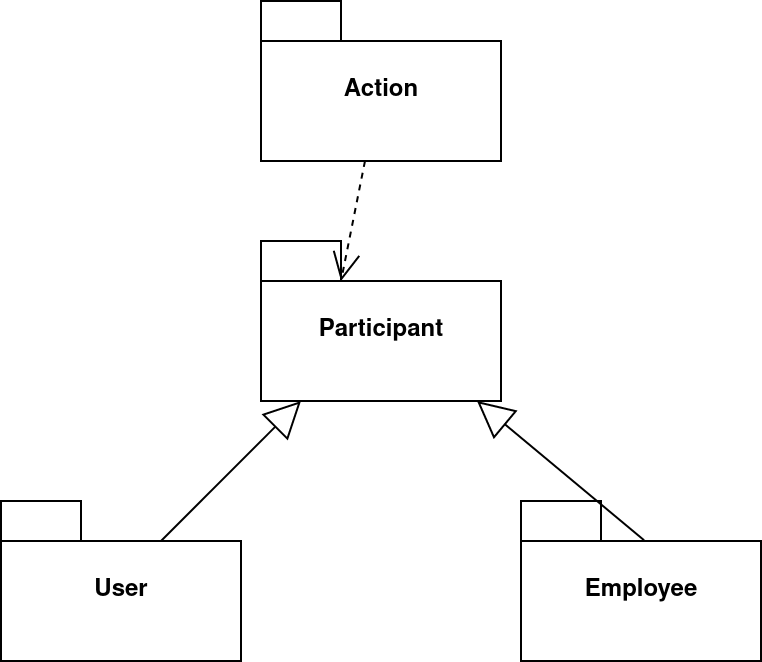
\includegraphics[scale=0.2]{pics/ex1.png}
            \caption{几个包的关系示意图}
            \label{figure:ex1}
        \end{figure}

        \pause
        这个例子展示了几个包之间的简单关系。
        
    
    \end{frame}

    \begin{frame}[fragile]
        \frametitle{SAP 的例子}
        
        对于 \verb|Participant| 这个包,如果不采用抽象,那么 \verb|Action| 在调用它做一些事情(比如说,个人信息采集等)的时候,将不得不

        需要额外的参数来区分它是 \verb|User| 还是 \verb|Employee|,这就增大了包的耦合性。\pause
    
        而如果采用抽象的方法,那么无论它具体是什么类型,\verb|Action| 在调用它的时候都只需要简单地调用 \verb|Participant| 中同一个类的同
        
        一个方法即可,无需额外传递参数,从而降低包的耦合性。
    
    \end{frame}

    \begin{frame}[fragile]
        \frametitle{SAP 的例子}

        而对于其他没有被依赖的包,比如说 \verb|User|,它没有被任何其他包所依赖,因此它应该具体。\pause
        
        否则,它的耦合度不一定会下降,但是一定会变得“毫无用处”。
    \end{frame}
\end{document}